\documentclass[conf]{new-aiaa}
%\documentclass[journal]{new-aiaa} for journal papers
\usepackage[utf8]{inputenc}

\usepackage{graphicx}
\usepackage{amsmath}
\usepackage[version=4]{mhchem}
\usepackage{listings}
\usepackage{color}
\usepackage{siunitx}
\usepackage{longtable,tabularx}
\usepackage{subcaption}
\usepackage{cleveref}
\usepackage{appendix}
\setlength\LTleft{0pt}

\title{Plot the Rankine Oval by using python code}

\author{Ranjithkumar B}
%\affil{SC22M008, M.Tech. Aerospace - Aerodynamics and Flight Mechanics}


\definecolor{mygreen}{rgb}{0,0.6,0}
\definecolor{mygray}{rgb}{0.5,0.5,0.5}
\definecolor{mymauve}{rgb}{0.58,0,0.82}

\lstset{
  backgroundcolor=\color{white},   % choose the background color; you must add \usepackage{color} or \usepackage{xcolor}; should come as last argument
  basicstyle=\footnotesize,        % the size of the fonts that are used for the code
  breakatwhitespace=false,         % sets if automatic breaks should only happen at whitespace
  breaklines=true,                 % sets automatic line breaking
  captionpos=b,                    % sets the caption-position to bottom
  commentstyle=\color{mygreen},    % comment style
  deletekeywords={...},            % if you want to delete keywords from the given language
  escapeinside={\%*}{*)},          % if you want to add LaTeX within your code
  extendedchars=true,              % lets you use non-ASCII characters; for 8-bits encodings only, does not work with UTF-8
  firstnumber=0001,                % start line enumeration with line 1000
  frame=single,                    % adds a frame around the code
  keepspaces=true,                 % keeps spaces in text, useful for keeping indentation of code (possibly needs columns=flexible)
  keywordstyle=\color{blue},       % keyword style
  language=Octave,                 % the language of the code
  morekeywords={*,...},            % if you want to add more keywords to the set
  numbers=left,                    % where to put the line-numbers; possible values are (none, left, right)
  numbersep=5pt,                   % how far the line-numbers are from the code
  numberstyle=\tiny\color{mygray}, % the style that is used for the line-numbers
  rulecolor=\color{black},         % if not set, the frame-color may be changed on line-breaks within not-black text (e.g. comments (green here))
  showspaces=false,                % show spaces everywhere adding particular underscores; it overrides 'showstringspaces'
  showstringspaces=false,          % underline spaces within strings only
  showtabs=false,                  % show tabs within strings adding particular underscores
  stepnumber=2,                    % the step between two line-numbers. If it's 1, each line will be numbered
  stringstyle=\color{mymauve},     % string literal style
  tabsize=2,                       % sets default tabsize to 2 spaces
  % title=\lstname                   % show the filename of files included with \lstinputlisting; also try caption instead of title
}

\begin{document}

\maketitle

%\section{Nomenclature}
%
%{\renewcommand\arraystretch{1.0}
%	\noindent\begin{longtable*}{@{}l @{\quad=\quad} l@{}}
%		$M$  & Free stream Mach number \\
%		$P$ &    Static pressure \\
%		$P_0$& Toatal pressure \\
%		$\gamma$ & Specific heat coefficient\\
%		$\theta$ & Flow turn angle \\
%		$ \beta $ & Wave angle \\
%		$ M_2$ & Downstream Mach Number\\
%		$ C_p$ & Coefficient of pressure \\
%		$\nu(M) $ & Prandt- Meyer Function
%\end{longtable*}}

% \begin{abstract}
%     This document contains the list of questions along with answers
%     given as tutorial - 01.
% \end{abstract}

\section{Problem Definition}
\par This work presents the solving potential flow equation (Rankine Oval) Numerically by using finite diffrence method, and compare those results with the Exact solution for understanding the FDM. \\

\section{Governing Equations}
\par Rankine Oval will be formed by combining the three two types of elementary flows, those are
\begin{enumerate}
	\item Uniform Flow (First elementary flow)
	\item Source and sink (Second elementary flow)
\end{enumerate}
\begin{figure}[!h]
    \center
    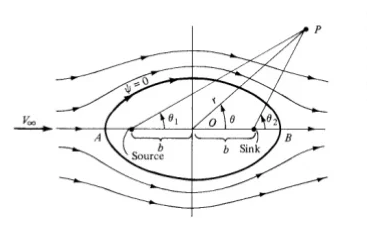
\includegraphics[scale=0.8]{images/oval.png}
    \caption{Flow over a Rankine oval}
    \label{fig01}
\end{figure}
\par Here the stream function equation is generally used for computing velocity components.\\
\begin{align*}
	\psi & = V_\infty r \sin{\theta} + \frac{\Lambda}{2 \pi} \theta_1 -\frac{\Lambda}{2 \pi} \theta_2\\
\end{align*}
\par By using the stream function, the Radial and Tangential velocities are\\
\begin{align*}
	u & = \frac{\partial \psi}{\partial y} \\
	v & = \frac{\partial \psi}{\partial x} \\
\end{align*}
\par The distance  between the souce to center and  sink to center should be same for Rankine oval. \\
\par Here the free stream velocity and source and sink strength are $V_\infty = 10 \ m/s$ and $\Lambda = 100 \ m^2/s $

\section{Numerical calculation}
\par By using finite diffrence method for solving the governing equation for 200 nodes for each direction.\\
\begin{align*}
	u & = \frac{\partial \psi}{\partial y} \\
	& = \frac{\psi_2 - \psi_1}{y_2-y_1} \\
	v & = \frac{\partial \psi}{\partial x} \\
	& = \frac{\psi_2 - \psi_1}{x_2-x_1} \\
\end{align*}
\par The above diffrence method only can solve or use $(N-1)$ grid only.For the last grid we use extrapolation method to get the velocity components.\\
\begin{align*}
	u_N & = 2 u_{N-1} - u_{N-2}\\
	v_N & = 2 v_{N-1} - v_{N-2}\\
\end{align*}

\section{Analytical calculation}
\par Based on the coordinates and flow condition itself the exact solution obtained by below Equations \\
\begin{align*}
	u & = V_\infty + \frac{\Lambda}{2 \pi} \left (\frac{X+b}{(X+b)^2+Y^2}-\frac{X-b}{(X-b)^2+Y^2} \right ) \\
	v & = \frac{\Lambda}{2 \pi} \left (\frac{Y}{(X+b)^2+Y^2}-\frac{Y}{(X-b)^2+Y^2} \right ) \\
\end{align*}
\par The X and Y denotes the co-ordinates from the center.Here the origin offset to (0.5,0.5) \\

\section{Solution and Observation}
\par The numerical and Eaxct solution was ploted in a single plot for the comparision purpose.\\
\begin{enumerate}
	\item For increaing the gid point, the accuracy of the solution also increase for certain limit.
	\item The orange stream lines are taken form the Analytical equation, and the Blue color stream lines are computed by numerical method.
	\item Those two streamlines are more over allined one on one in the figure \ref{fig02}.
\end{enumerate}

\begin{figure}[!h]
	\center
	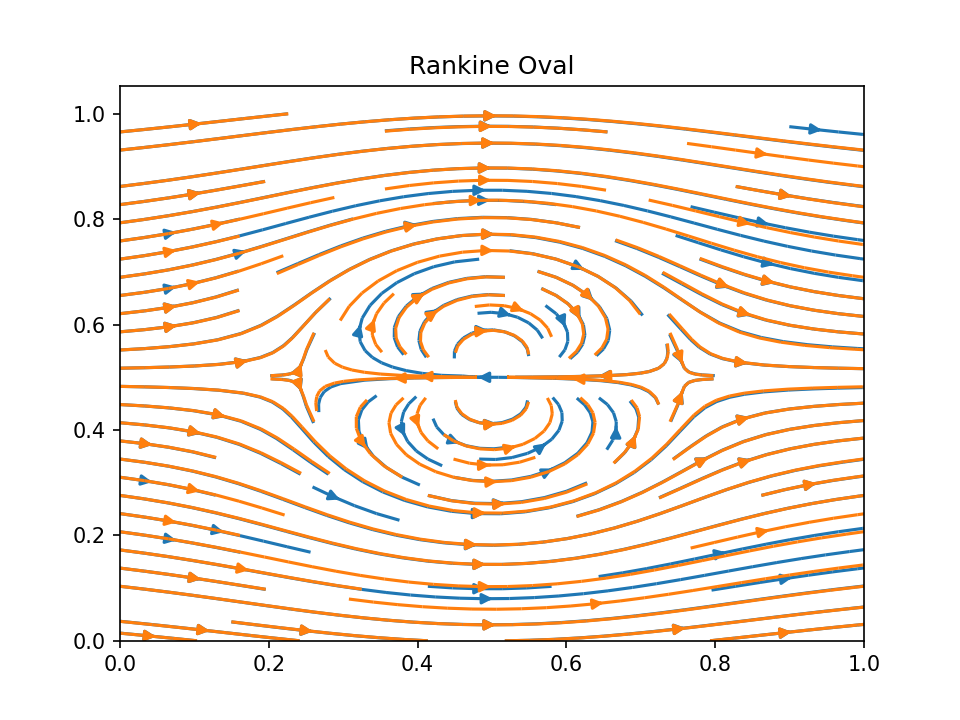
\includegraphics[scale=0.8]{images/Result.png}
	\caption{Numerical and exact solution of Rankine oval}
	\label{fig02}
\end{figure}
\pagebreak

\begin{thebibliography}{9}
    \bibitem{ref_1} Jhon D Anderson Jr., "Fundamentals of Aerosynamics," Fifth Edision 2010.
    \bibitem{ref_2} Jhon D Anderson Jr., "Computational Fluid Dynamics The basics with applications,"Indian edition
\end{thebibliography}

\pagebreak
 \begin{appendices}
      \section{Appendix - Python code}\label{appendixA}
      This section contains the \emph{Python} code of Rankine Oval.
     
      \lstinputlisting{Code/Rankine_Oval.py}
     
      \pagebreak
 \end{appendices}

\end{document}
